\chapter{Question-Asking and Plan Inference}
\label{ch:question_plan}
\textbf{Salena Torres Ashton, Stephen Kim, Loren Rieffer-Champlin, Liang Zhang,
Adarsh Pyarelal, Clayton Morrison}


\section{Summer 2022 Introduction}

While academic researchers focus on theoretical and epistemological questions, primary school teachers may focus more on pedagogical questions, and professional researchers in industry may use all three types of questions. All three of these situations assume cooperative dialog and optimal information-sharing between conversation partners, in most case\footnote{This paper makes the same assumption: all question and natural language discourse evaluations assume cooperative dialog and intent, epistemological questions and the mutual goal of optimal (or at least maximal) information-sharing.} Adversarial or interrogative questions, often accompanied with minimal or evasive information-sharing dialog, tend to be the norm for law enforcement professions. In either case, how a question is asked is often more important than what questions are asked \citet{ray_2001}. When we ask questions that reflect our goal, purpose, or confusion,  we strengthen relationships, increase productivity and learning, and create an equitable environment \citet{rothe_lake_gureckis_2018} and \citet{alaimi_2020}. We reduce transaction \footnote{I define transaction costs as the cost of anything that is to be done, regardless of outcome or goal. Opportunity costs are the costs to do one action at the mutual exclusion of not having the opportunity to do the other action.} and opportunity costs imposed on relationships or business opportunities. Question-asking, and not just question-answering, minimize these costs because they clarify goals and intentions between dialog partners.

Artificial Intelligence (AI), Information Retrieval, and Natural Language Processing yield exciting research into question-\emph{answering}, relevant document retrieval, Theory of Mind (ToM), and human-computer interaction. However, the literature is sparse within the  \emph{intersection} of artificial intelligence, psycho linguistics, indirect speech acts, negative knowledge modeling, ToM, and question-\emph{asking}. Hawkins and Goodman address this sparsity and the trend of past research to focus on the optimization of question-answering, not question-asking \citet{hawkins_goodman_2017}. 

\subsection{Question-Asking, Goal Inference and Urban Search and Rescue Communication}
This paper investigates the gap between question-asking natural language discourse and player goals through goal inference using video observations of teams who play Minecraft in an urban search and rescue scenario. Video observations of teams playing together in this SAR scenario were annotated using procedural Grounded Theory. In the SAR scenario implemented for ASIST Study 3, teams of human players
engage in cooperative behavior to search for, stabilize, and rescue victims
within a collapsed building. As human players verbalize plans, make
suggestions, or tell each other what to do, they also ask questions that can
infer hidden goals or intentions. Teammates reduce their individual knowledge
asymmetry by asking and answering questions. Due to the cost of human annotation efforts, Twelve video observations were annotated for this study.Preliminary results warrant continued research using a larger sample size and human annotation effort. The results of this study show that teams who ask more questions at a more consistent rate and with the intent to collaborate lead to better team performance than teams who ask fewer questions, ask more how-to questions, or use questions as a polite way to give directions to teammates. I then conclude with a discussion of future research based on these conclusions. 

\subsection{Gricean Maxims and Indirect Speech Act}
People are generally free to ask epistemological questions in cooperative dialog settings. People can choose how much they want to follow social conventions when phrasing questions. Indirect Speech Act Theory details social conventions that we generally follow when asking and answering questions. Informative (i.e., “I have an appointment at five. Do you have the time?”) and uninformative questions where I only ask for the time \citet{clark_1979}. When I ask you, “Do you have the time?” I do not expect, nor would I appreciate your answer of, “Yes.” Though the answer is logically correct, it is considered rude.

The Gricean Maxims affirm our purposes of conversation: to formalize language and to keep language informal \citet{grice_1975}. Formal language has truth values that are easy to identify. When asked if we have the time, we either do or we do not have the time.However, when we formalize natural language, we obscure or disregard the full purpose of communication. Grice explains the unwritten rules of acceptable informal language known as \emph{implicature}, through maxims,  assume cooperative dialog, have a common purpose and accept dialog turn-taking\citet{grice_1975}. These social convention, generally state that conversation is best when we say no more or no less information than is required, tell the truth, do not speculate, be relevant, avoid ambiguity, be orderly, and be polite. A blatant violation of these maxims would be a question like, "\emph{When is it? Why can't you remember anything?}" There is not enough information, the subject is ambiguous, the delivery is neither polite nor orderly, and implies that the listener is not good at listening or remembering details. Less blatant violations would be questions like, "\emph{What day do we go there?}" This question is ambiguous because of its co-reference without context. This ambiguity can be reduced through the study and application of question-asking. 





\subsection{SIGNIFICANCE}

Not understanding goal or intention can be seen in the designs of artificial intelligence agents who are programmed with researcher bias. If that AI agent's purpose is to assist humans in a SAR scenario, the programmer and researcher must check (or augment) their own domain knowledge of SAR communications in order to curb their biases toward academic best practices regarding the programming of uncertainty, belief and reinforcement learning. The understanding of SAR communications is vital for the programmers in AI fields in order to design a realistic and scalable domain. The cost of programming AI agents for SAR task execution-- but not studying\footnote{or consulting SAR experts.} the information-gathering habits of real-life human rescue workers can result in flawed domains that predict human player and AI agent action or intent at no better than chance. 

Therefore, question-asking and information-sharing is vital in a domain definition of a Search and Rescue scenario (SAR) just as much as it is in real life. The INSARAG marking system\footnote{FEMA has a similar marking but is only used in the United States, whereas INSARAG is used internationally.} is designed to immediately answer the most frequently-asked questions a rescuer will have in an urban SAR disaster: Go or No-Go, number of live victims, number of dead victims, number of unaccounted-for victims, hazards, building floor references, cleared areas of building, and cleared building \citet{insarag_2022}. SAR workers further communicate with each other through radio, sound horns and Morse code, and direct communication with victims and each other.

Answering these anticipated, frequent questions could be programmed using formalism or rule-based logic-- and that has been the standard practice for question asking until recently. 


\subsection{LITERATURE}
\subsubsection{Goals, Intentions, and Listeners}
When we ask questions, we are not seeded with a set of questions or handed a set of 'correct and incorrect' questions. We do not prefer questions with literal, logical answers \citet{rothe_lake_gureckis_2017} and \citet{clark_1979}. However, most research has focused on answer sets or query matching, preference for concise
questions and answers. In reality, people ask open-ended questions, sloppy half questions, use questions to politely tell others what to do, and meander in speech without
purpose \citet{brown_1980}. We ask questions to express goals. 

Goals reflect a desired endpoint or world state. A goal can be motivated by belief, desire or intent. People ask questions that either express a goal or infer a hidden goal. 
A question is the interpretation and response of a hidden (or uttered) goal to be discerned
by another person, typically a dialog partner \citet{hawkins_goodman_2017}. Indirect speech acts and question-answer dialog is a form
of \emph{information asymmetry}: a questioner has a goal but needs information,
while an answerer has information but does not know the questioner’s goal. Missing or contradictory information naturally leads to a knowledge goal and the generation of questions. The person is then motivated to ask a question \citet{alaimi_2020}. 

Intentions demonstrate action choice to reach that goal-- it is reflected in the way a question is to be asked. A questioner believes that the listener’s knowledge base has information that can facilitate the questioner’s goal. 
The type of questions then asked will depend on context, social inference, and other signals in a dialog setting. The key is to 
decouple\footnote{Hawkins and Goodman's 2017 work was limited to epistemological questions and cooperative behavior.} the inferred goal from the explicit meaning of the question \citet{hawkins_goodman_2017}. This redefinition of \emph{What is a Question} enables models to account for context and avoid assumptions. 

Questions can be viewed as a hidden goal or intent, but they can also be viewed as a way to provide or reinforce knowledge \citet{alaimi_2020} and \citet{ray_2001}. Question-askers want the listener to directly understand their goal, or to discern a hidden goal, or both-- then to give appropriate responses (however that appropriate response may be for the context). When question-askers do not receive appropriate answers from listeners, both dialog partners use conversational implicature and politeness to reach a mutual understanding. They will minimize potential transaction and opportunity costs in conversation to reach mutual understanding.  

\subsubsection{Formal Language Representation}
Formal language representation for this paper must represent a problem in an abstract symbology or representation, consist of an ontology, have intelligent reasoning, be effective at computation, and be capable of mimicking human expression at some level \citet{DavisR}. Knowledge representation for natural language suggests the formalization of words, phrases, and context but the computational aspects do not capture the fuller meaning or purpose of why natural language exists at all. Ultimately, this means that using logic or answerset programming to investigate question-asking and question-answering will be computationally efficient, but neither sound nor complete enough for human beings. Language formalism can be used to generate open-ended questions and investigate their semantic representations by creating a probabilistic generative model that uses importance sampling, Expected Information Gain and Shannon entropy \citet{rothe_lake_gureckis_2017}. Treating questions as programs to model question-asking in humans, then executing the question ‘programs’ upon a world to receive output as an answers or generated questions resulted in models that can predict what humans will ask. These models also create novel questions not found in training sets and can produce human-like questions\citet{rothe_lake_gureckis_2017}. Rothe concluded that people choose which questions to ask by balancing the amount of information to be gained and the complexity of asking such a question. 

\subsubsection{Free-form Natural Language}
Free-form natural language, as opposed to rule-based logics, and Bayesian updating models account for human behavioral and computations experimentation when investigating question-asking behaviors. People prefer to ask good-enough questions instead of complex or optimal information gathering questions. People are good at identifying good questions but have a hard time asking good questions \citet{rothe_lake_gureckis_2018} when they are unfamiliar with the tools or have no practice in asking questions. These findings support the works of \citet{alaimi_2020}, \citet{hawkins_goodman_2017}, \citet{ray_2001}.

Though the current literature on psycho-linguistics and question-asking is sparse, what is consistently available are the everyday experiences of project leaders, business managers, family members, customer service representatives and teachers who are surrounded by curious and bright people who set goals, reach goals, and ask questions. They are equally surrounded by the bright and curious who may have a goal and knowledge gap, but do not ask questions. When dialog partners do not or cannot minimize the costs required to obtain mutual understanding, the previous assumption of cooperative dialog, unconstrained phrasing, and epistemological questions is no longer valid, thus introducing the above-mentioned transaction and opportunity costs.





\section{Spring 2022 Introduction}

In the SAR scenario implemented for ASIST Study 3, teams of human players
engage in cooperative behavior to search for, stabilize, and rescue victims
within a collapsed building. As human players verbalize plans, make
suggestions, or tell each other what to do, they also ask questions that can
infer hidden goals or intentions. Teammates reduce their individual knowledge
asymmetry by asking and answering questions.  We will investigate how uttered
questions can infer another person's goal or intention. 

This investigation will guide future research into knowledge engineering and
representation of tasks, goals, and hidden intentions. While simple human goals
may be represented with classical AI planning, we believe that complex goals with 
constraints or multiple levels of abstraction may be best
represented by a \emph{hierarchical task network} (HTN)\ap{Add a definition of
HTN here}, which is a tree of possible
plans.\footnote{Technically, the plans produced by HTN planners can also be
    represented with flat lists - however, in this section, we use the term
`plan' to refer to the actual `plan tree' that contains the task decompositions
as well, rather than just the plan alone.}

We will investigate the following research questions for Study 3:

\begin{enumerate}
    \item How do spoken questions reveal another person's plan or intent? 
    \item Can people listen to spoken questions and accurately decide if the
        other person's plan is sequential or hierarchical? Can the
        distinction between such structures improve predictive performance for
        Artificial Social Intelligence (ASI) agent intervention?
\end{enumerate}

%%%%%

The current literature for the intersection of theory of mind (ToM) and
question-\emph{asking} is sparse. \citet{hawkins_goodman_2017} address this
scarcity and the trend of past research to focus on the optimization of
answer-giving, usually through answer sets or query matching.  prefer concise
questions and answers. However, in reality, people do not ask questions
expecting an answer from a predetermined set of answers.
They may ask open-ended questions, meander in speech without
purpose, and use indirect speech acts to express mutual goals or build rapport
with each other. 

\cite{hawkins_goodman_2017} connect question-asking and intention
\emph{because} of the scarcity of ``empirical evidence about how social context
affects the questioner’s choice." They redefined the meaning of a question as
"the interpretation and response of a hidden (or uttered) goal, to be discerned
by another person, typically a dialog partner"\ap{Where is this from? Is it
verbatim?} \citep{hawkins_goodman_2017}.
Hawkins and Goodman describe speech acts and question-answer dialog as a form
of \emph{information asymmetry}: a questioner has a goal but needs information,
while an answerer has information but does not know the questioner’s goal. The
type of questions then asked will depend on context, social inference, and
signals in a dialog setting. The significance of their work is in the
decoupling of the inferred goal from the explicit meaning of the question. This
helps model context and avoid assumptions \footnote{Their work was limited to
epistemic questions and cooperative behavior.}.

Examining someone's answer to a question rather than the question itself may be
another way to understand intent. While \cite{hawkings_goodman_2017} define questions as
hidden goals or intentions, Mehdi Alaima et al\ap{use citet} define the act of asking
questions as ‘the providing of information or knowledge to reinforce knowledge
one way or another,"\ap{fix mismatched quotes, check whether this is verbatim.} independently paralleling the definition given by Hawkins
and Goodman \ap{use citet}. "When information is missing, or contradicts what one knows, a
knowledge goal will arise, often leading to the generation of questions. The
person is then made aware of the information needs, and motivated to formulate
a question to obtain the missing knowledge,” \citep{alaimi_2020}\ap{fix
reference}. Building on
the claims of Hawkins and Goodman\ap{citet}, and Alaima et al\ap{citet}, we investigate
question-asking within the SAR scenario of ASIST’s Minecraft environment. 


\section{Approach}

We assume that questions have hidden goals and infer plans. As teams ask more
questions of each other, human team ToM converges toward cooperative behavior.
We will investigate whether question-asking is associated with \emph{team
planning}, defined as a set of goals, strategies, or tasks that are executed.
We define \emph{coordination} as behaviors and utterances to create a common
plan or strategy\footnote{Note that this is distinct from the mathematical
definition of coordination proposed in \autoref{ch:pgm}}. We define
\emph{cooperation} as team behaviors that implement an already-agreed up on
plan.

To capture hidden goals, inferred plans, and patterns that may represent human
ToM, we will annotate six ASIST Study 3 Spiral 2 pilot video observations and
six HSR ASIST Study 3 videos released between March 29 and May 5, for a total
of at least twelve videos. These videos are of three distinct missions for each
team. Due to the expensive costs of taxonomy label development with strict
adherence to grounded theory methodology, this stage of the experiment is
limited to no less than twelve videos. 

Two human annotators will code all uttered questions between teammates within
the Minecraft SAR scenario.  We use the qualitative coding procedure known as
Grounded Theory, as defined by \citet{corbin_strauss_2015}. 

More specifically, and as defined by \citet{saldana_2021}, we will use a
Grounded Theory Process Coding for a state or action across some interval of
time. These \emph{grounded-in-data} labels are known as \emph{concept-level}
labels, which are the smallest pieces of data that encode a question-asking
phenomena of interest.

More specifically, and as defined by \citet{saldana_2021}, we will use a
Grounded Theory Process Coding for a state or action across some interval of
time. These \emph{grounded-in-data} labels are known as \emph{concept-level}
labels, which are the smallest pieces of data that encode a question-asking
phenomena of interest. We also use this coding methodology to investigate the connectivity and
causality of each concept label to discover possible relationships between
presence or absence of team actions, interactions, conditions, and consequences
of question-asking. Densely-connected concept labels suggest subcategories and
categories. Sparsely-connected labels will not be discarded; they will be used
to consider variability within patterns and categories that emerge. In cases
where questions have co-reference or other contextual dependencies, only that
direct dependency will be coded for local semantic meaning.

We make the following considerations when creating codes: 

\begin{itemize}
    \item Frequency will not dictate importance, causality, or connectivity of a concept
    \item Each question will have at least one annotation and up to four
      annotations:
    \begin{itemize}
        \item Primitive actions (ground truth). Ex: breakRubble,
          requestStabilizedVictimCarry.
        \item Abstraction Levels of actions (of primitive actions) Respective
          examples: respondRubbleRequest or createVictimAccess, collaborateStabilizedVictim
    \end{itemize}
    \item Labels will be stemmed and minimally normalized
    \item Capturing the phenomena of question-asking across time, between any subset of a team, between the same team across the two different missions. 
\end{itemize}


To avoid annotator and researcher biases and any \emph{a priori} belief on
which team ToM strategies may be used, concept and category labels are not
pre-determined. Inter-annotator agreement must reach a Kappa Score of 80\% or
higher. This also gives a more solid, grounded analytical meaning to any
emergent categories. 

After the development of labels and taxonomy, the investigation of team ToM and
question-asking will scale for additional videos. When all concepts,
subcategories, categories can reasonably explain the phenomena of the video
observations, one or two super-categories, \emph{theories of team plan}, will
emerge. We currently assume that a theory of team plan would have greater
predictive power and ToM inference potential. 


\section{Evaluation}

Because of the small sample size of this investigation, we will not perform a
quantitative evaluation at this time. Instead, we will perform a qualitative
investigation of word frequencies, clustering patterns, and correlation of
annotator-generated labels through data visualization. Below is a list of
possible visualizations we may consider:

\begin{itemize}

    \item Connectivity of concept-level labels: radial diagrams, arc diagrams,
        matrix diagrams or graph networks

    \item Frequency patterns of words or concept labels (normalized, word count
        / total number of words in that question): scatterplots or histograms

    \item Correlation of words and labels with time: time series, scatterplots. 

    \item Concept-level subcategorization(s): clustering, PCA (concept labels
        possibly projected onto sub-categorical spaces), or hierarchical
        visualizations.

\end{itemize}


Such visualizations, based on twelve videos, will lead to further insight
through this investigation. Future measures may include Mann-Whitney U-Tests,
t-tests (only if we annotate a large-enough sample), precision and recall of
the concept-level and category patterns to describe the generalizability for
real data with no ASI interventions, generalizability for real data with ASI
interventions, and the variance of patterns in label categories. Another
possible measure, for future research, would be the F1 score to explain how
well these labels describe observations without ASI interventions, when
compared to high-intervention observations. This future investigation would
address measure ASI-M5: Coordinative Communications to
measure teamwork, include additional video observations for real data in Study
3, and continue our investigation of whether human plans and ToM are best
represented by classical planning or HTN planning.


\section{Summer 2022 Results, Conclusions, Discussion and Future Research}
\subsection{Preliminary Results}
\subsubsection{Label Development and Annotation}

I used a bottom-up Grounded Theory qualitative coding method to investigate connections between a question-asker's intention and words spoken. This
rigorous theory ensures that my work is not biased, as it uses unsupervised
labels and does not lend itself to the proof or disproof of prior researcher
belief in Minecraft SAR player strategy. This data-driven, robust method
captures player intention, team strategy, and naturally lends itself to
quantitative analysis. Videos were selected from no-human intervention videos,
at random, and three teams were chosen as a sequence (team 217, 218 and 219).
Two independent annotators\footnote{Salena Ashton, PhD Student, School of Information, University of Arizona; and Stephen Kim, MS Information Science} annotated six study-3 pilot
videos with unconstrained, not-previously-determined labels. 

The continuous disambiguation
of unsupervised labels, using lexical definitions, led to extensive
documentation of words to be used as labels for the capturing of specific
phenomena in observations.\footnote{For example, when an annotator should use
the verb 'ask', 'clarify', or 'request'.} We then constrained labels for real
data in two ways only: format the label in 'verbObjectObject' camelCase and use
the lexical definition to avoid ambiguous use of any word. Beyond these two
requirements, annotators were free to create any label desired to code a
player's question. We then annotated six different study-3 real data
videos\footnote{Salena Ashton and Loren Reiffer-Champlin, both PhD Students, School of Information, University of Arizona}, which then lead to Theoretical
Saturation \footnote{Theoretical saturation is the point when few additional
labels are created, regardless of fully-autonomous annotators' ability to
create new ones. Saturation demonstrates that the existing label schema fully
capture the events and phenomena observed.} and converged around 21 verb
labels, 24 noun labels, 25 modifier labels. Without replacement, these
components can yield 12,600 possible labels, yet we demonstrated theoretical
saturation through the independent construction of less than 100 labels from
two autonomous annotators.


\subsubsection{Annotator Agreement}
We achieved an unweighted Cohen Kappa\footnote{Grounded Theory is robust in its
unsupervised labeling approach is because annotators have complete autonomy.
Because the sample size is small, the theoretical probability of two matching
labels is even smaller, and only two annotators worked on the real data, there
is no current justification for using Scott's pi or a weighted Kappa. This will
change as further research scales.} agreement of 0.892. Using the
disambiguation documentation and Merriam-Webster's Dictionary to meticulously
settle any annotator label disagreement, we declared the question labels as
'agree' or 'disagree'. When annotator intention and the disambiguation
documentation did not clarify the agreement or disagreement of labels, we
declared it as 'disagreement'. 


\subsubsection{Emergent Categories}

About 100 labels resulted from real data annotations and were analyzed for
emergent categories and preliminary patterns. Label frequency \emph{did not}
dictate importance. Data visualization and preliminary analysis focus on three
key features: \emph{questionLabel}\footnote{Qualitative code representation of the
question utterance and no further context except for co-reference resolution.
Some questions were spoken as statements with inflection. Other questions were
actually demands shrouded with politeness. All three types of questions were
coded for this investigation. All questions asked are assumed to be uttered
with cooperative intent.}, \emph{abstractLabel}\footnote{Code representation of
player intention. This was captured by taking the question into context. For
example, if the question were represented by 'requestBreakRubble', the intent
behind the question could have been 'collaborateCriticalWake' or
'navigateLocation'. AbstractLabel is not the representation of *why* a
question had been asked; it is the *intention* of the player who asked the
question.}, and \emph{utterance}, the word of interest uttered in a question. From
the emergent categories, we chose specific words that did or *did not*
represent player interaction\footnote{For example: *ask*, *request*,
*suggest*, and *clarify* are all actions that show the goal of
obtaining information, but 'clarify' asks for additional information after the
initial question, showing two-way dialog, 'request' is an initiation of
commitment to another player with the optional accept/ reject response, showing
two-way dialog. 'Suggest' also initiates like 'request' but does not give the
option to accept or reject, making the question and dialog a one-way
discussion. 'Ask' is a one-way dialog utterance to obtain information.}. 

The following themes emerge from the data:

\begin{itemize}
    \item Less Team Collaboration (talking \emph{at or to} a teammate and not \emph{with} a teammate)
    \begin{itemize}
    	\item Labels that include: direct, suggest, inform, etc.
	\item Word utterances: go, I see, there are, and other phrases that inform but do not invite collaboration
    \end{itemize}
    \item More Team Collaboration (talking \emph{with} a teammate)
    \begin{itemize}
        \item Labels that include: ask, request, answer, clarify, teammate, coordinate, collaborate, plan, wake
        \item Word utterances: can you, should we, you guys, what do you think, let's, wake, this time
    \end{itemize}
    \item Intention toward position: location or destination, but not necessarily navigation strategies.
    \item Prioritizing an idea: plan, suggest, request, collaborate, critical, or any victim.
    \item Question utterances that were actually demands (do you mind doing...; why don't you go and clear...). This indicates conversation implicature and politeness, as described by the Gricean Maxims and Gretchen Brown.
    \item Statements that were questions with inflection, and other nuanced utterances: suggest, tell, direct, request; context and explanations included in annotation.
\end{itemize}










\newpage
\subsection{Figures for Labels}
\subsubsection{Question Utterances Joint Probabilities}
%%% Start figure 1%%%%%%%%%%%%%%%%%%%%%%%%%%%%%%%%%%%%%%%%%%%%%%%%
%ggsave(filename = "figures/questionLabelProbability_STA.pdf")
\begin{figure}[h!]
    \centering
    \fbox{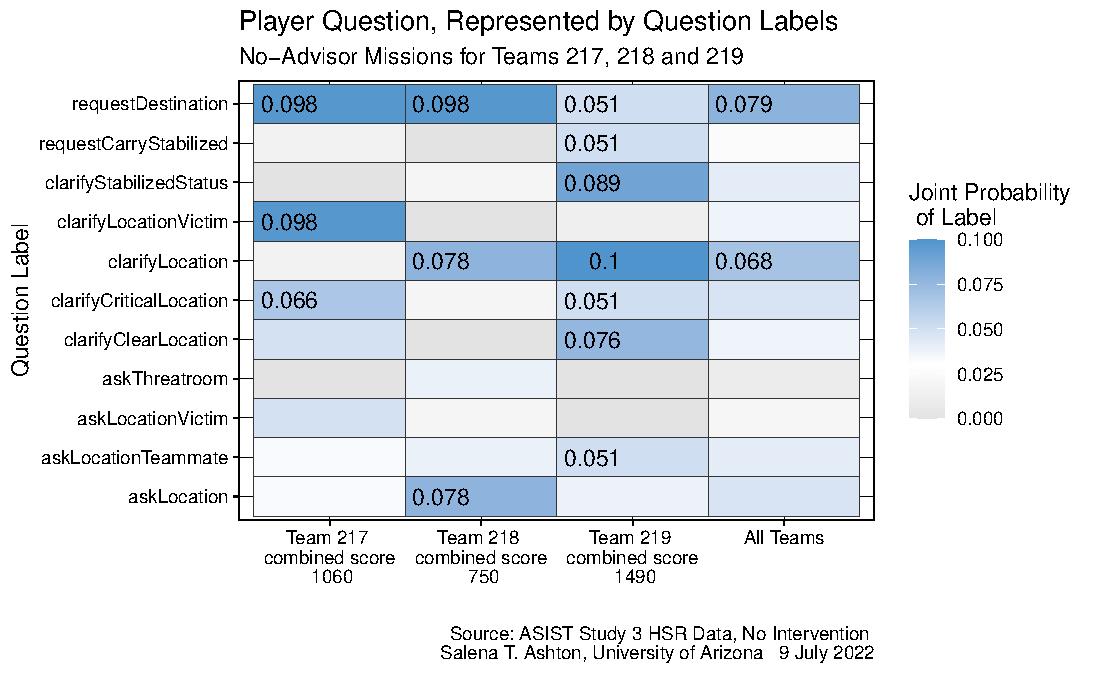
\includegraphics[width=0.9\textwidth]{../images/questionLabelProbability_STA.pdf}}
    \caption{Figure 1: Teams who scored higher tended to ask questions about the collaboration of victims, whereas teams who did not score as high asked questions about location or destination (where destination is a location that is a goal).}
\end{figure}
%%%% Above figure is updated 6 Sept 2022 %%%%%%
% End figure 1%%%%%%%%%%%%%%%%%%%%%%%%%%%%%%%%%%%%%%%%%%%%%%%%








\newpage
%start fig 2 %%%%%%%%%%%%%%%%%%%%%%%%%%%%%%%%%%%%%%%%%%%%%%%
%ggsave(filename = "figures/abstractLabelProbability_STA.pdf")

\begin{figure}[h!]
    \centering
    \fbox{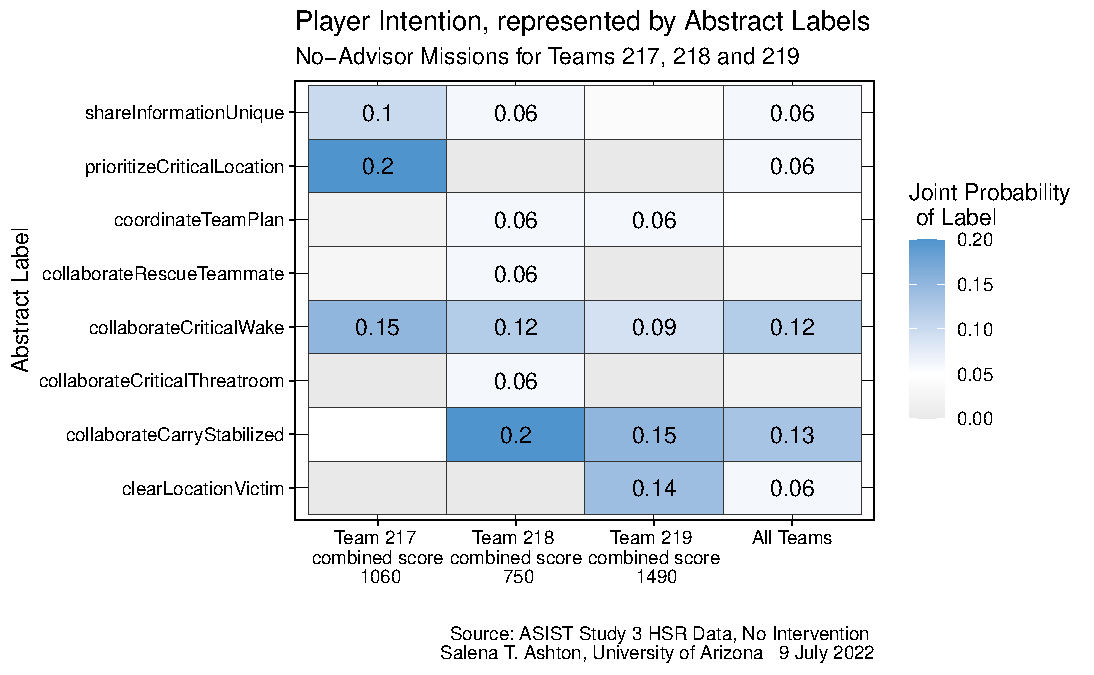
\includegraphics[width=0.9\textwidth]{../images/abstractLabelProbability_STA.pdf}}
    \caption{Figure 2: Player intention (represented by abstract labels) is an unobserved, inferred behavior. Ground-truth question utterances demonstrate team collaboration differently than abstract labels.}
\end{figure}
%%%% Above figure is updated 6 Sept 2022 %%%%%%%%%%%%%%%%%%%%%%%%%%%%%%%%%%%%
% End figure 2%%%%%%%%%%%%%%%%%%%%%%%%%%%%%%%%%%%%%%%%%%%%%%%%








\newpage
%start fig 3 %%%%%%%%%%%%%%%%%%%%%%%%%%%%%%%%%%%%%%%%%%%%%%%
\subsubsection{ Player Intention, given the Question Asked}
%ggsave(filename = "figures/abstractLabel_ConditionalProbability_STA.pdf")



\begin{figure}[h!]
    \centering
    \fbox{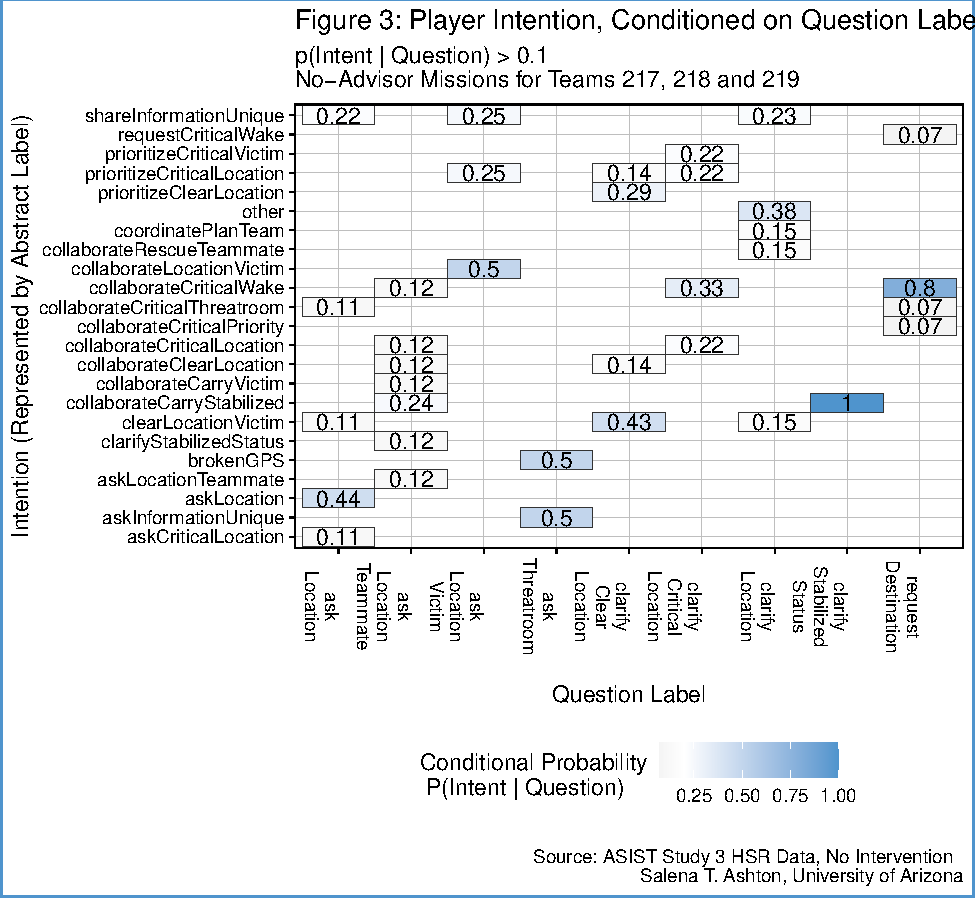
\includegraphics[width=0.9\textwidth]{../images/abstractLabel_ConditionalProbability_STA.pdf}}
    \caption{Figure 3: When we look at the question that was asked, we are able to predict their intentions only part of the time. Though we cannot conclude that questions will always predict intention from this small study, we can see that further research with a larger sample size is warranted. Patterns that emerge include that given question utterance 'requestDestination', the player's intent is more than 80\% likely to be waking a critical victim. Human annotators intuitively agree with this assessment.}
\end{figure}
%%%% Above figure is updated 6 Sept 2022 %%%%%%%%%%%%%%%%%%%%%%%%%%%%%%%%%%%%
% End figure 3%%%%%%%%%%%%%%%%%%%%%%%%%%%%%%%%%%%%%%%%%%%%%%%%








\newpage
%start fig 4 %%%%%%%%%%%%%%%%%%%%%%%%%%%%%%%%%%%%%%%%%%%%%%%

\subsubsection{Questions Asked, given the Player Intention}
%ggsave(filename = "figures/questionLabel_ConditionalProbability_STA.pdf")

\begin{figure}[h!]
    \centering
    \fbox{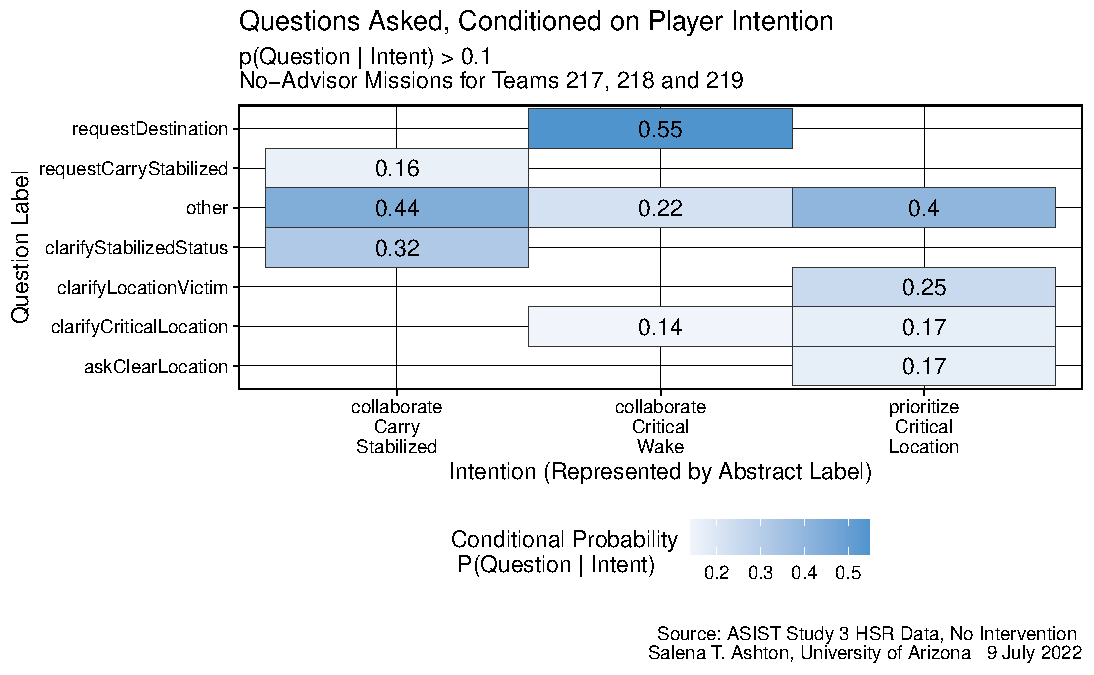
\includegraphics[width=0.9\textwidth]{../images/questionLabel_ConditionalProbability_STA.pdf}}
    \caption{Figure 4: Three player intention themes emerge when all possible intentions are filtered for more than 10\%: collaborateCarryStabilized, collaborateCriticalWake, and prioritizeCriticalLocation. When a player's intention is to wake a critical, they are 55\% likely to ask another player to join
 them ('requestDestination'). This observation is trivial because the game rules state that at least two people are needed to wake a critical. However, the previous figure shows the flipped conditions: a player's intention is more than 80\% likely to be waking a critical when 'requestDestination' is asked. When teams collaborate to wake a critical victim, they request or clarify --not suggest or tell-- a teammate to come to a particular destination. ('Clarify' and 'request' infer two-way dialog of commitment creation whereas 'direct' or 'suggest' are creation commitments or demands that do not give the listener a chance to respond.) }
\end{figure}
%%%% Above figure is updated 6 Sept 2022 %%%%%%%%%%%%%%%%%%%%%%%%%%%%%%%%%%%%
% End figure 4%%%%%%%%%%%%%%%%%%%%%%%%%%%%%%%%%%%%%%%%%%%%%%%%








\newpage
%start fig 5 %%%%%%%%%%%%%%%%%%%%%%%%%%%%%%%%%%%%%%%%%%%%%%%

\subsubsection{Question Frequency and Consistency}
%ggsave(filename = "figures/QuestionTiming_STA.pdf")




\begin{figure}[h!]
    \centering
    \fbox{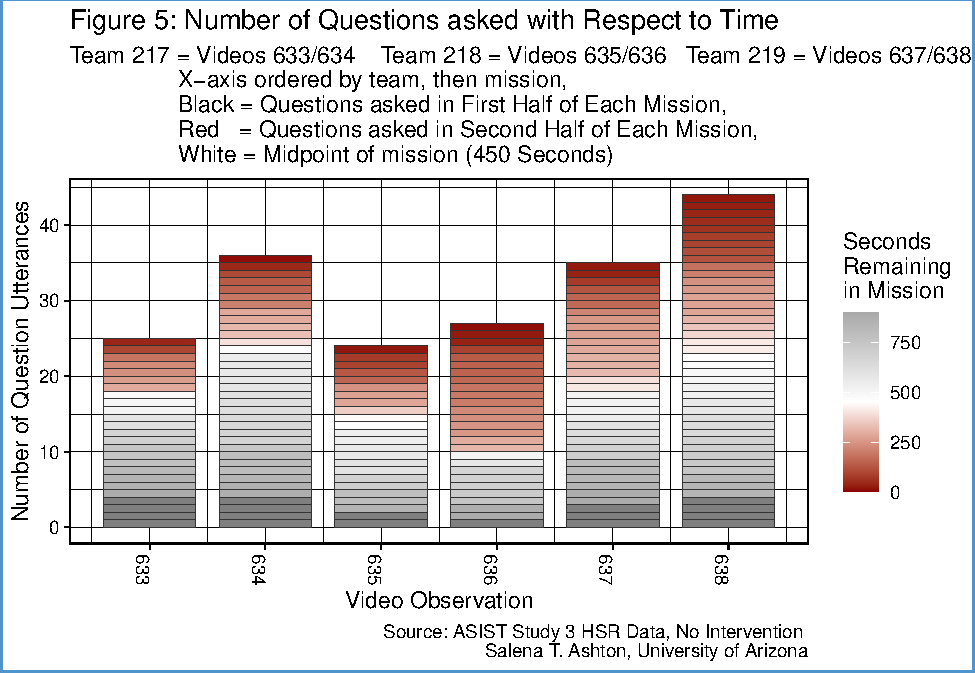
\includegraphics[width=0.9\textwidth]{../images/QuestionTiming_STA.pdf}}
    \caption{Figure 5 displays time as color. As show, team 218 (videos 635 and 636) asked the
fewest questions, scored the lowest combined points, and asked 66\%
of questions toward the end of the mission. This suggests that teams who score poorly tend to ask fewer questions that focus on collaboration or planning-- and more questions that ask specific task-oriented items toward the end of each mission. Team 3 (videos 637 and 638) asked the most questions and asked questions at a \emph{consistent rate} throughout their missions. This suggests that teams who score higher tend to ask questions at a consistent rate, enabling the exchange of information, building of rapport and team trust, and setting a social convention of asking each other for collaboration or help. }
\end{figure}
% End figure 5%%%%%%%%%%%%%%%%%%%%%%%%%%%%%%%%%%%%%%%%%%%%%%%%








\newpage
%start fig 6 %%%%%%%%%%%%%%%%%%%%%%%%%%%%%%%%%%%%%%%%%%%%%%%

\subsubsection{Player Intentions, given the Word Utterance}
%  labs(title = "Figure 6: Player Intentions Given the Words Used in Question-Asking",
 %    subtitle = "p(Intention | Word Utterance) > 0.1 ",
%     caption = "Source: ASIST Study 3 HSR Data, No Intervention \nSalena T. Ashton, University of Arizona",
%     y = "Player Intention",
%     x = "Word Uttered in Question",
%     fill = "p(Intention | Word Utterance)") +
%ggsave(filename = "figures/QuestionUtterances_Link_STA.pdf")





\begin{figure}[h!]
    \centering
    \fbox{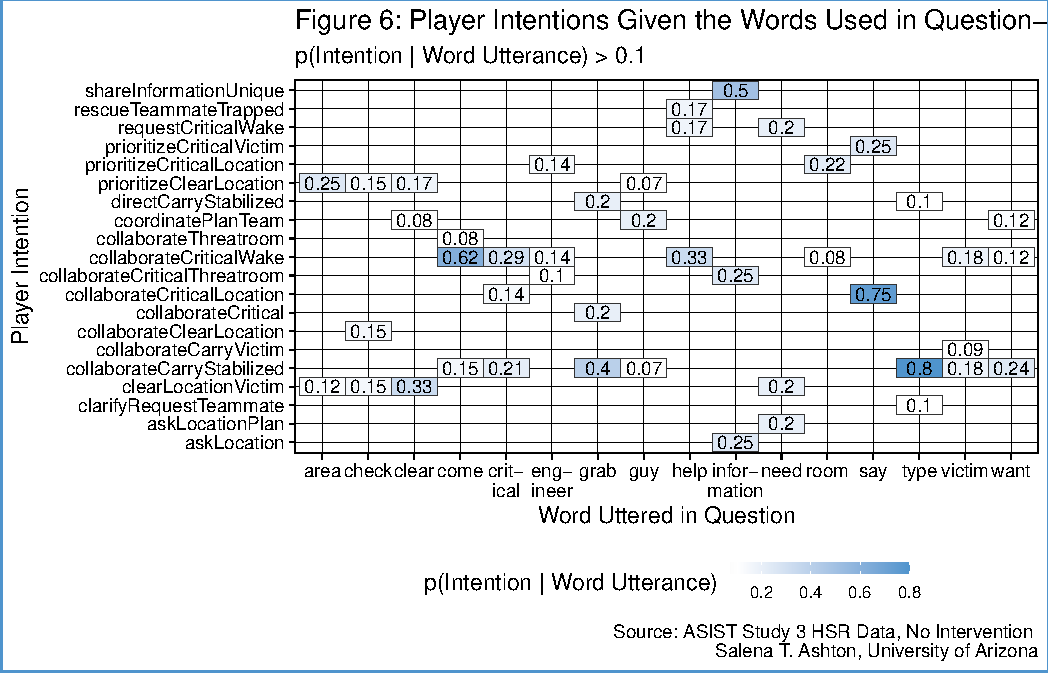
\includegraphics[width=0.9\textwidth]{../images/QuestionUtterances_Link_STA.pdf}}
    \caption{Figure 6: Non-domain-specific words that show collaboration include: say, type, or come. These conclusions were made using the 1 x 1 Bag of Words algorithm and matched to intention by hand. The \textbf{significance} of this figure shows that a priori researcher bias can be harmful when designing a domain. For example, our team previously believed that words like: navigate, location, victim, room, critical and marker were the most important words to look for when inferring player intention. This figures shows that is not the case. A priori research team error: navigate, location, victim, room, critical, marker, or area.}
    \end{figure}
    
   
\begin{comment}
Corrected research team information regarding Player Intention:
\begin{itemize}
    \item 'Come' infers team collaboration for waking up a critical victim
    \item 'Grab' infers team collaboration for carrying victims that have been healed
    \item 'Say' infers team collaboration of locating critical victims
    \item 'Type' infers team collaborating for carrying victims that have been healed
\end{itemize}
\end{comment}

% End figure 6%%%%%%%%%%%%%%%%%%%%%%%%%%%%%%%%%%%%%%%%%%%%%%%%








\newpage
%start fig 7 %%%%%%%%%%%%%%%%%%%%%%%%%%%%%%%%%%%%%%%%%%%%%%%

\subsubsection{Word Utterance, given Player Intention}

%ggsave(filename = "figures/Intent_to_Utterances_Link_STA.pdf")

\begin{figure}[h!]
    \centering
    \fbox{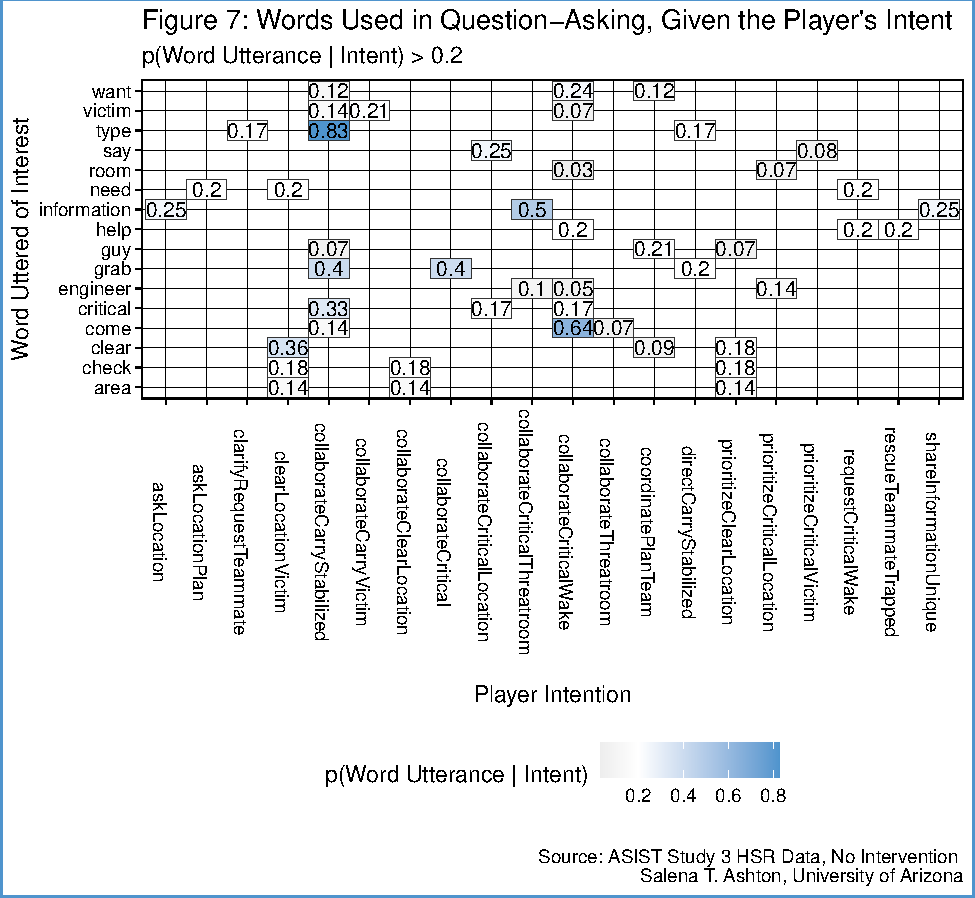
\includegraphics[width=0.9\textwidth]{../images/Intent_to_Utterances_Link_STA.pdf}}
    \caption{Figure 7: Players who work together tend to say  'come', 'say' (stemmed), 'type' or 'want.' When they work together to carry victims, they will most likely say 'type' (or mark) to identify the victim type. As shown, the emergence of a possibly-interesting pattern, especially when non-domain words like 'type' show a strong correlation to specific intentions. The \textbf{significance} of this figure demonstrates how plan-recognition researchers may consider such non domain-specific words when designing a domain.
}
\end{figure}
% End figure 7%%%%%%%%%%%%%%%%%%%%%%%%%%%%%%%%%%%%%%%%%%%%%%%%








\newpage
%start fig 1 smoothed %%%%%%%%%%%%%%%%%%%%%%%%%%%%%%%%%%%%%%%%%%%%%%%
\subsubsection{Smoothed Granularity: Player Intention, given the Question Asked}

%ggsave(filename = "figures/SMOOTHED_abstractLabel_ConditionalProbability_STA.pdf")

\begin{figure}[h!]
    \centering
    \fbox{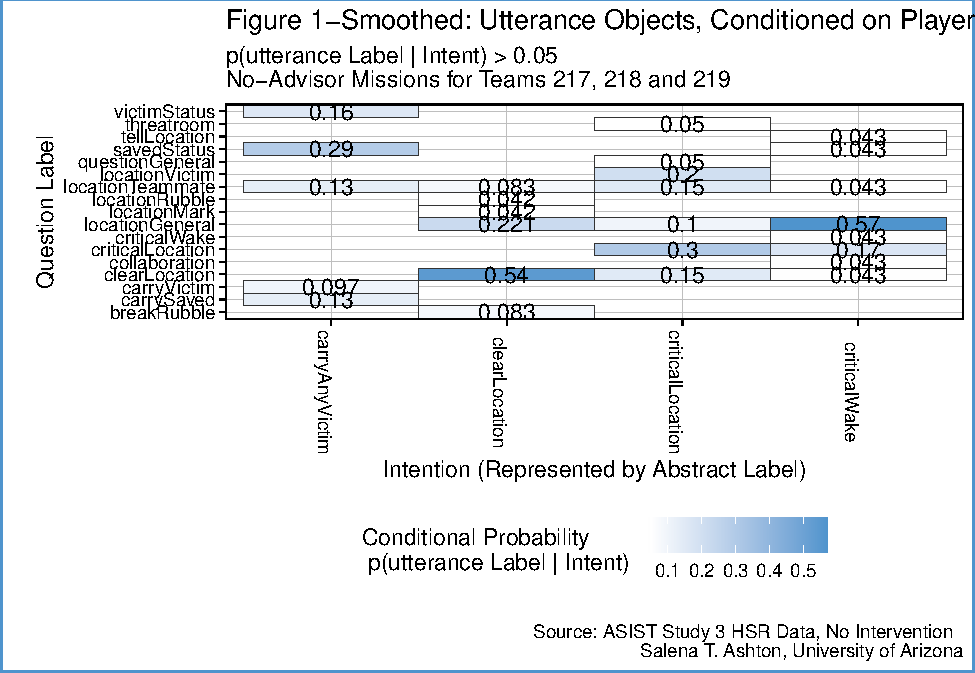
\includegraphics[width=0.9\textwidth]{../images/SMOOTHED_abstractLabel_ConditionalProbability_STA.pdf}}
    \caption{Figure 1 smoothed: When we look at the question that was asked, we are able to predict their intentions only part of the time. Though we cannot conclude that questions will always predict intention from this small study, we can see that further research with a larger sample size is warranted. Patterns that emerge include that given question utterance 'requestDestination', the player's intent is more than 80\% likely to be waking a critical victim. Human annotators intuitively agree with this assessment.}
\end{figure}
% End figure 1 smoothed%%%%%%%%%%%%%%%%%%%%%%%%%%%%%%%%%%%%%%%%%%%%%%%%








\newpage
%start fig 4 smoothed%%%%%%%%%%%%%%%%%%%%%%%%%%%%%%%%%%%%%%%%%%%%%%%

\subsubsection{Smoothed Granularity: Questions Asked, given the Player Intention}
%ggsave(filename = "figures/questionLabel_ConditionalProbability_STA.pdf")

\begin{figure}[h!]
    \centering
    \fbox{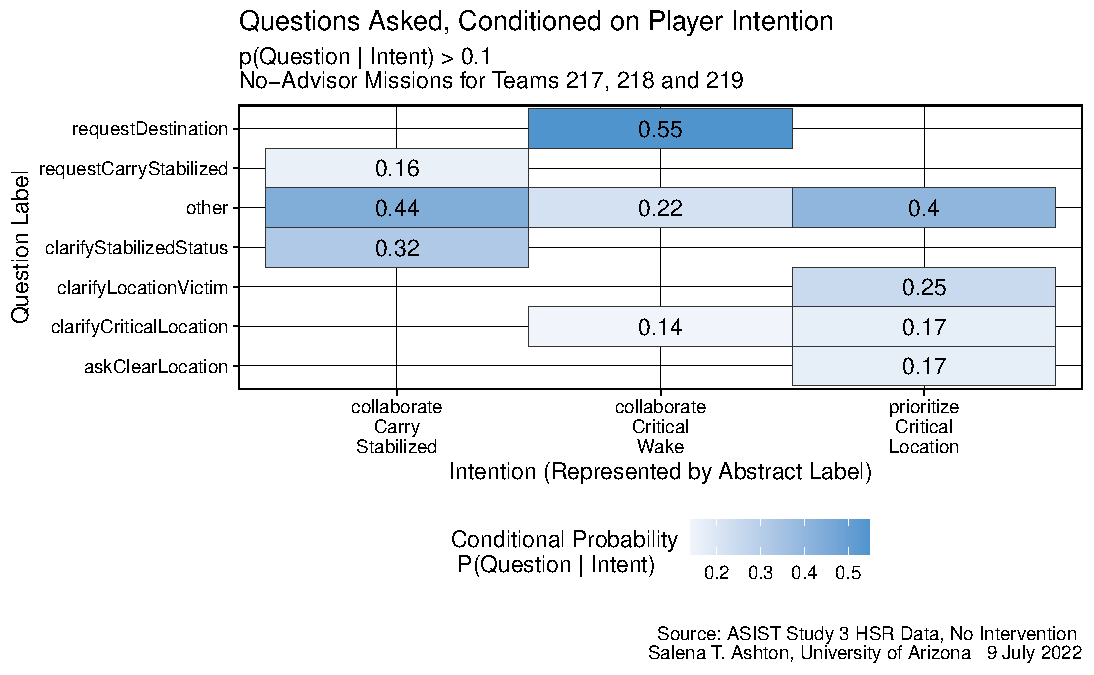
\includegraphics[width=0.9\textwidth]{../images/questionLabel_ConditionalProbability_STA.pdf}}
    \caption{Figure 4 smoothed: Three player intention themes emerge when all possible intentions are filtered for more than 10\%: collaborateCarryStabilized, collaborateCriticalWake, and prioritizeCriticalLocation. When a player's intention is to wake a critical, they are 55\% likely to ask another player to join
 them ('requestDestination'). This observation is trivial because the game rules state that at least two people are needed to wake a critical. However, the previous figure shows the flipped conditions: a player's intention is more than 80\% likely to be waking a critical when 'requestDestination' is asked. When teams collaborate to wake a critical victim, they request or clarify --not suggest or tell-- a teammate to come to a particular destination. ('Clarify' and 'request' infer two-way dialog of commitment creation whereas 'direct' or 'suggest' are creation commitments or demands that do not give the listener a chance to respond.)}
\end{figure}
% End figure 4 smoothed %%%%%%%%%%%%%%%%%%%%%%%%%%%%%%%%%%%%%%%%%%%%%%%%








\newpage
%start fig 8 %%%%%%%%%%%%%%%%%%%%%%%%%%%%%%%%%%%%%%%%%%%%%%%

\subsubsection{Connections to Natural Language Utterance Using Trigrams}

The ultimate goals of this registration are two-fold: find evidence to (1)
continue the investigation of intent, given a question being asked, using
causal reasoning and other approaches (2) develop algorithms to extract this
intent from utterance transcriptions of player without human annotator
dependency. We believe that emergent categories that result from these 12 video
annotations do *warrant* continued investigation, which would include the
following possible tasks:

\begin{itemize}
    \item Scale for additional data: Ashton is currently building a model that maps words\footnote{Bag of Words and other models, at word and sentence level.} and intentions.
    \item Natural generation model: Use the above model to re-create the labels
        generated by Ashton and Reiffer-Champlin. We will compare these results
        to model labels with the taxonomy developed by ODIN and the Dialog
        Agent at the University of Arizona.
    \item Additional human annotation of data; compare models in earlier stages to these results until the automation of linking intention with natural language is credible and reproducible.
    \item Compare and contrast emerging team ToM from no-intervention observations to high-intervention observations.
    \item Quantitative analyses and causal inference models.
\end{itemize}

%ggsave(filename = "figures/trigram_Utterances_STA.pdf")


\begin{figure}[h!]
    \centering
    \fbox{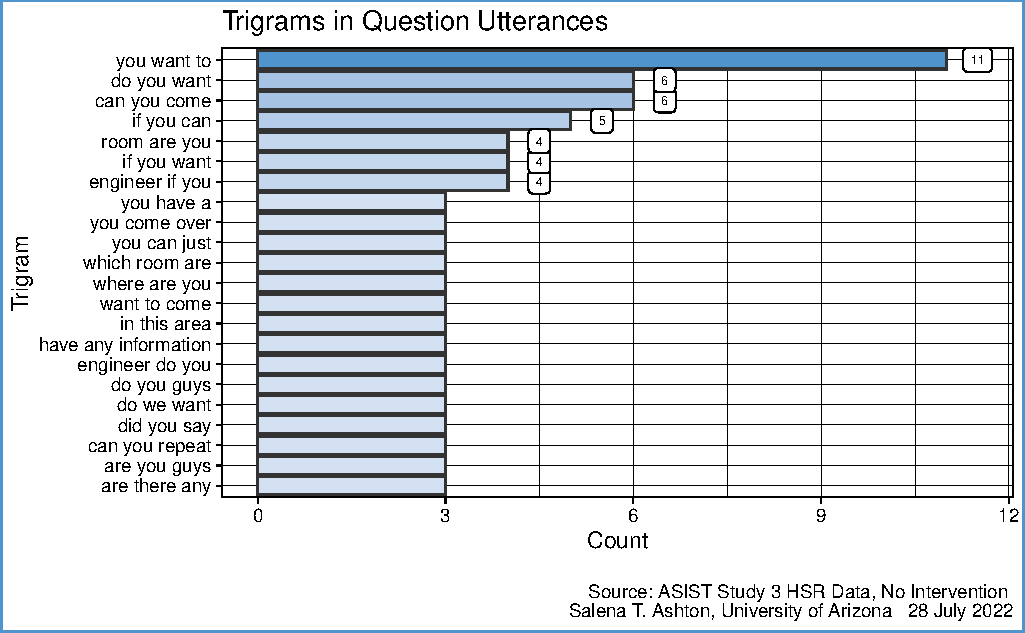
\includegraphics[width=0.9\textwidth]{../images/trigram_Utterances_STA.pdf}}
    \caption{Using the Python package NLTK, I extracted the most common N-grams of the players' question utterances (for all teams, N = 3). When I first did this, there were no interesting patterns. I then removed the "English" library of stopwords to be removed and found the following patterns. This yields exciting potential for further research into the logical argument and flow of player intention. For example, the word "if" shows a conditional statement from one player to another. "If you can..." was a common utterance but it was also a polite imperative, not a request or question. The phrase "do you guys" and "do we want" to not carry as much information about named entities, but it does show ample collaboration of teammates. }
\end{figure}
% End figure 8%%%%%%%%%%%%%%%%%%%%%%%%%%%%%%%%%%%%%%%%%%%%%%%%








\newpage
%start fig 9 and 10 %%%%%%%%%%%%%%%%%%%%%%%%%%%%%%%%%%%%%%%%%%%%%%%

 %ggsave(filename = "figures/FINAL_1_trigram_Utterances_STA.pdf")


\begin{figure}[h!]
    \centering
    \fbox{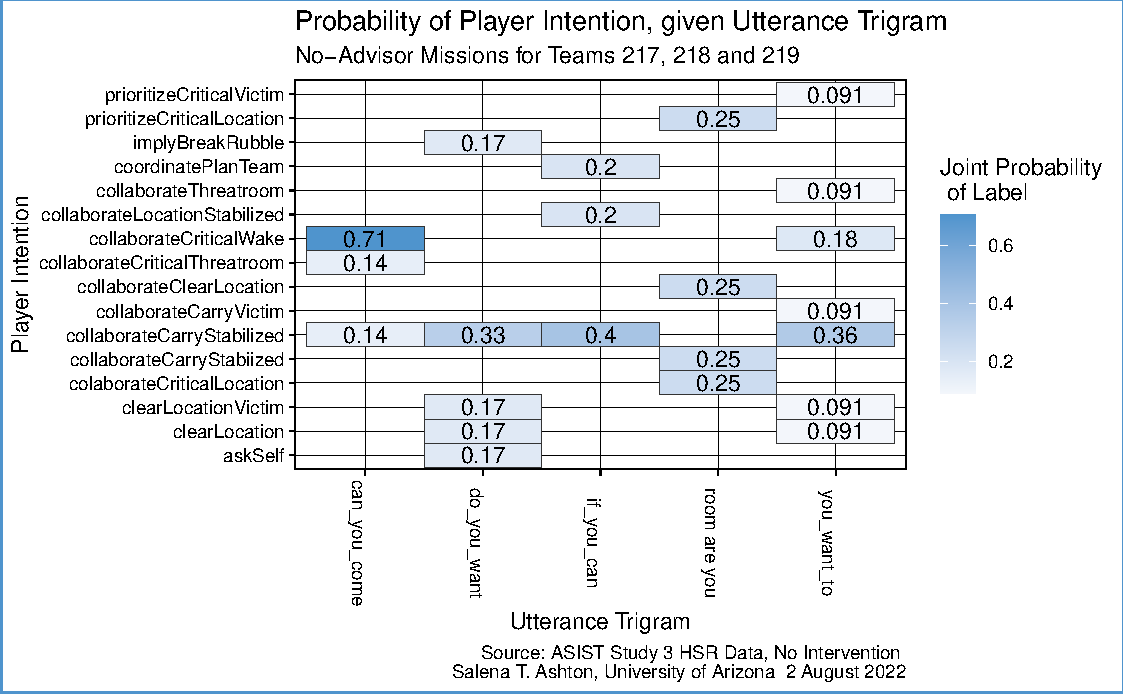
\includegraphics[width=0.9\textwidth]{../images/FINAL_1_trigram_Utterances_STA.pdf}}
    \caption{Figure 9}
\end{figure}




%  labs(title = "Figure 10: Probability of Trigram Utterance, given Player Intent",
  %   subtitle = "No-Advisor Missions for Teams 217, 218 and 219",
    % caption = "Source: ASIST Study 3 HSR Data, No Intervention \nSalena T. Ashton, University of Arizona  2 August 2022",
     %y = "Utterance Trigram",
%     x = "\nPlayer Intention",
 %    fill = "Joint Probability\n of Label") +
%ggsave(filename = "figures/FINAL_2_trigram_Utterances_STA.pdf")


\begin{figure}[h!]
    \centering
    \fbox{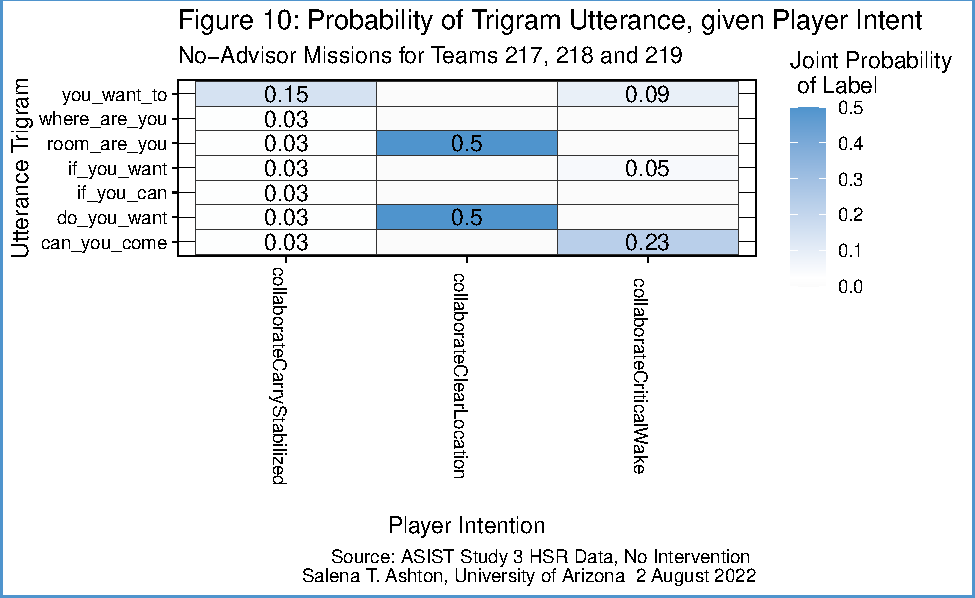
\includegraphics[width=0.9\textwidth]{../images/FINAL_2_trigram_Utterances_STA.pdf}}
    \caption{Figures 9 and 10 show \emph{quantitatively} shows that players will explicitly collaborate with each other, explicitly state their individual and team goals, hedge their imperatives when working in cooperative situations, and will even show when teams choose \emph{not} to cooperate, as is the case when "can you just"-- a less-polite way of telling someone what to do.
}
\end{figure}
% End figure 9 and 10%%%%%%%%%%%%%%%%%%%%%%%%%%%%%%%%%%%%%%%%%%%%%%%%



\newpage

\subsection{CONCLUSION}
In this paper, I have discussed how questions can infer explicitly-stated goals, inferred goals, and how questions are better understood through indirect speech acts. I then use a Search and Rescue scenario within ASIST's Minecraft Environment to evaluate how teammates will ask each other questions in order to make and reach individual and team goals. These goals and player intentions were captured with a robust and vigorous coding process called Grounded Theory, annotated by two completely-autonomous annotators, and reached an unweighted Kappa Cohen score of 0.892. I then investigated these data through a series of visualizations, joint and conditional probabilities, and mapping the data to natural language utterances. This preliminary study has two significant limitations: Only twelve videos were annotated for questions. Future research must include the annotation of many more videos, their questions and non-questions. 

\subsubsection{Significant findings}
\begin{itemize}
    \item Previous researcher belief that players create intentions around domain-specific words are not supported in this research
    \item Previous top-down domain definition of the Search and Rescue yielded results that were no better than chance. This preliminary study shows several inferences that fair better than chance for player intention, questions asked, and natural language of questions that are asked.
    \item Teams demonstrate collaboration through non domain-specific words like 'come', 'say' and 'type'.
    \item Stops words that are traditionally removed for natural language processing must be considered when infering goals or intentions toward team collaboration. Furthermore, it is these stop words that show the logical inference of such plans.
\end{itemize}


\subsection{Future Research}
I have found that further research is warranted for the investigation of question-asking, goal-setting, goal-reaching, and team collaboration. As a bonus, I have discovered that the stop-words not only hold potential research investigation for the logical flow of such arguments, but can possibly yield new insight into causal inference and reasoning\footnote{It is my intention to continue this line of research for a directed research study in Fall 2022 (Causal Inference) and in Spring 2023 (Comprehensive Qualification Exam for my PhD program in Information Science at the University of Arizona).} It is my hope that the findings of this preliminary study and future research will have significant application toward continued work for the ToMCAT- ASIST program \footnote{Theory of Mind-based Cognitive Architecture for Teams (ToMCAT), Natural Language Generation for Artificial Intelligence and Planning Task \# 7} and for continued study of probabilistic and causal reasoning. 

\newpage






\section{Spring 2022 Results}

\subsection{Label Development, Annotation and Annotator Agreement}

We used a bottom-up Grounded Theory qualitative coding method to investigate
any connections between a question-asker's intention and words spoken. This
rigorous theory ensures that our work is not biased, as it uses unsupervised
labels and does not lend itself to the proof or disproof of prior researcher
belief in Minecraft SAR player strategy. This data-driven, robust method
captures player intention, team strategy, and naturally lends itself to
quantitative analysis. Videos were selected from no-human intervention videos,
at random, and three teams were chosen as a sequence (team 217, 218 and 219).
Two independent annotators\footnote{Ashton and Kim} annotated six study-3 pilot
videos with unconstrained, unsupervised labels. The continuous disambiguation
of unsupervised labels, using lexical definitions, led to extensive
documentation of words to be used as labels for the capturing of specific
phenomena in observations.\footnote{For example, when an annotator should use
the verb 'ask', 'clarify', or 'request'.} We then constrained labels for real
data in two ways only: format the label in 'verbObjectObject' camelCase and use
the lexical definition to avoid ambiguous use of any word. Beyond these two
requirements, annotators were free to create any label desired to code a
player's question. We then annotated six different study-3 real data
videos\footnote{Ashton and Reiffer-Champlin}, which then lead to Theoretical
Saturation \footnote{Theoretical saturation is the point when few additional
labels are created, regardless of fully-autonomous annotators' ability to
create new ones. Saturation demonstrates that the existing label schema fully
capture the events and phenomena observed.} and converged around 21 verb
labels, 24 noun labels, 25 modifier labels. Without replacement, these
components can yield 12,600 possible labels, yet we demonstrated theoretical
saturation through the independent construction of less than 100 labels from
two autonomous annotators.

We achieved an unweighted Cohen Kappa\footnote{Grounded Theory is robust in its
unsupervised labeling approach is because annotators have complete autonomy.
Because the sample size is small, the theoretical probability of two matching
labels is even smaller, and only two annotators worked on the real data, there
is no current justification for using Scott's pi or a weighted Kappa. This will
change as further research scales.} agreement of 0.892. Using the
disambiguation documentation and Merriam-Webster's Dictionary to meticulously
settle any annotator label disagreement, we declared the question labels as
'agree' or 'disagree'. When annotator intention and the disambiguation
documentation did not clarify the agreement or disagreement of labels, we
declared it as 'disagreement'. 


\subsection{Emergent Categories, Team Theories, and Preliminary Patterns}

About 100 labels resulted from real data annotations and were analyzed for
emergent categories and preliminary patterns. Label frequency \emph{did not}
dictate importance. Data visualization and preliminary analysis focus on three
key features: 'questionLabel'\footnote{Qualitative code representation of the
question utterance and no further context except for co-reference resolution.
Some questions were spoken as statements with inflection. Other questions were
actually demands shrouded with politeness. All three types of questions were
coded for this investigation. All questions asked are assumed to be uttered
with cooperative intent.}, 'abstractLabel'\footnote{Code representation of
player intention. This was captured by taking the question into context. For
example, if the question were represented by 'requestBreakRubble', the intent
behind the question could have been 'collaborateCriticalWake' or
'navigateLocation'. AbstractLabel is not the representation of \emph{why} a
question had been asked; it is the \emph{intention} of the player who asked the
question.}, and 'utterance', the word of interest uttered in a question. From
the emergent categories, we chose specific words that did or \emph{did not}
represent player interaction\footnote{For example: \emph{ask}, \emph{request},
\emph{suggest}, and \emph{clarify} are all actions that show the goal of
obtaining information, but 'clarify' asks for additional information after the
initial question, showing two-way dialog, 'request' is an initiation of
commitment to another player with the optional accept/ reject response, showing
two-way dialog. 'Suggest' also initiates like 'request' but does not give the
option to accept or reject, making the question and dialog a one-way
discussion. 'Ask' is a one-way dialog utterance to obtain information.}. 

The following themes emerge from the data:

\begin{itemize}
    \item Less Team Collaboration (talking \emph{at or to} a teammate and not \emph{with} a teammate)
    \begin{itemize}
    	\item Labels that include: direct, suggest, inform, etc.
	\item Word utterances: go, I see, there are, and other phrases that inform but do not invite collaboration
    \end{itemize}
    \item More Team Collaboration (talking \emph{with} a teammate)
    \begin{itemize}
        \item Labels that include: ask, request, answer, clarify, teammate, coordinate, collaborate, plan, wake
        \item Word utterances: can you, should we, you guys, what do you think, let's, wake, this time
    \end{itemize}
    \item Intention toward position: location or destination, but not necessarily navigation strategies.
    \item Prioritizing an idea: plan, suggest, request, collaborate, critical, or any victim.
    \item Question utterances that were actually demands (do you mind doing...; why don't you go and clear...)
    \item Statements that were questions with inflection, and other nuanced utterances: suggest, tell, direct, request; context and explanations included in annotation.
\end{itemize}


\subsection{Discussion and Future Research}

The ultimate goals of this registration are two-fold: find evidence to (1)
continue the investigation of intent, given a question being asked, using
causal reasoning and other approaches (2) develop algorithms to extract this
intent from utterance transcriptions of player without human annotator
dependency. We believe that emergent categories that result from these 12 video
annotations do \emph{warrant} continued investigation, which would include the
following possible tasks:

\begin{itemize}
    \item Scale for additional data: Ashton is currently building a model that maps words\footnote{Bag of Words and other models, at word and sentence level.} and intentions.
    \item Natural generation model: Use the above model to re-create the labels
        generated by Ashton and Reiffer-Champlin. We will compare these results
        to model labels with the taxonomy developed by ODIN and the Dialog
        Agent at the University of Arizona.
    \item Additional human annotation of data; compare models in earlier stages to these results until the automation of linking intention with natural language is credible and reproducible.
    \item Compare and contrast emerging team ToM from no-intervention observations to high-intervention observations.
    \item Quantitative analyses and causal inference models.
\end{itemize}



\section{Figures and Additional Preliminary Analyses}
%%%%%%%%%%%%%%% Visuals  %%%%%%%%%%%%

% Question-Timing
\begin{figure}[h!]
    \centering
    \fbox{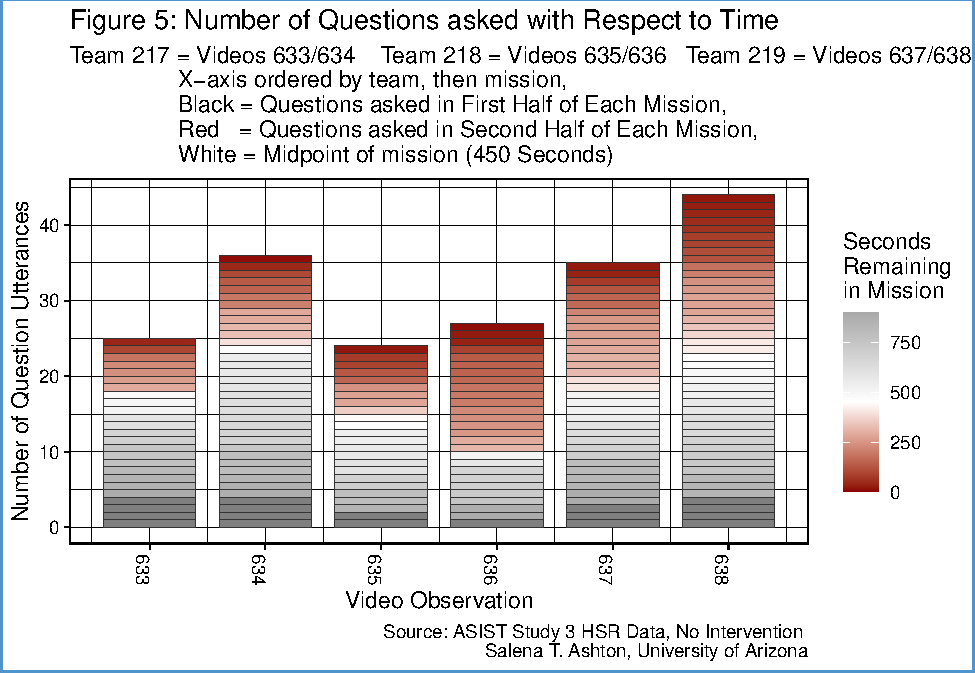
\includegraphics[width=0.9\textwidth]{../images/QuestionTiming_STA.pdf}}
    \caption{Time = color within histogram. Team 218 (videos 635 and 636) asked the
        fewest questions, scored the lowest combined points, and asked 66\%
        of questions toward the end of the mission. Team 3 (videos 637 and 638) asked
        the most questions and asked questions at a \emph{consistent rate} throughout their missions.}
    \end{figure}
    

% p(Question | Intent)
\begin{figure}[h!]
    \centering
    \fbox{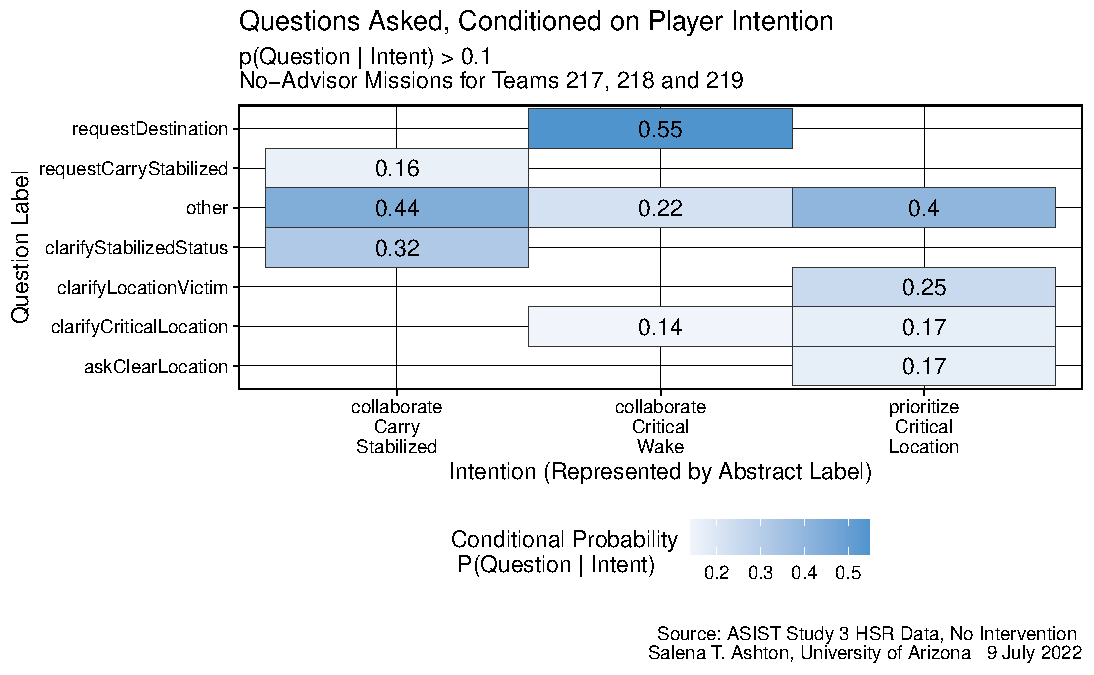
\includegraphics[width=0.9\textwidth]{../images/questionLabel_ConditionalProbability_STA.pdf}}
    \caption{Probabilities of questions to be asked center on three intentions (see figure). When teams collaborate to wake a critical victim, they request or clarify --not suggest or tell-- a teammate to come to a particular destination.('Clarify' and 'request' infer two-way dialog of commitment creation whereas 'direct' or 'suggest' are creation commitments or demands that do not give the listener a chance to respond.)}
\end{figure}

%p(Intent | Question)
\begin{figure}[h!]
    \centering
    \fbox{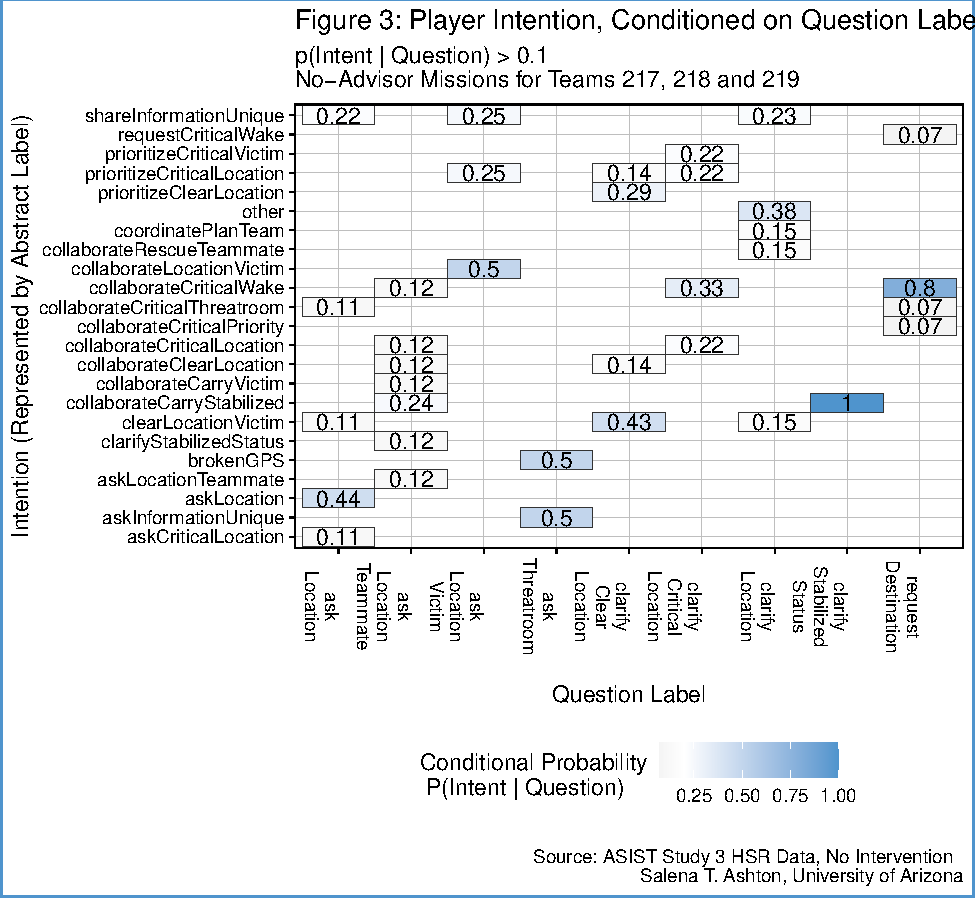
\includegraphics[width=0.9\textwidth]{../images/abstractLabel_ConditionalProbability_STA.pdf}}
    \caption{When a player's intention is to
        wake a critical, they are 55\% likely to ask another player to join
        them (trivial). Yet given question utterance 'requestDestination', the intent is more than 80\% likely to be waking a critical victim. }
\end{figure}


    
% p(Word Utterance | Intent)
\begin{figure}[h!]
    \centering
    \fbox{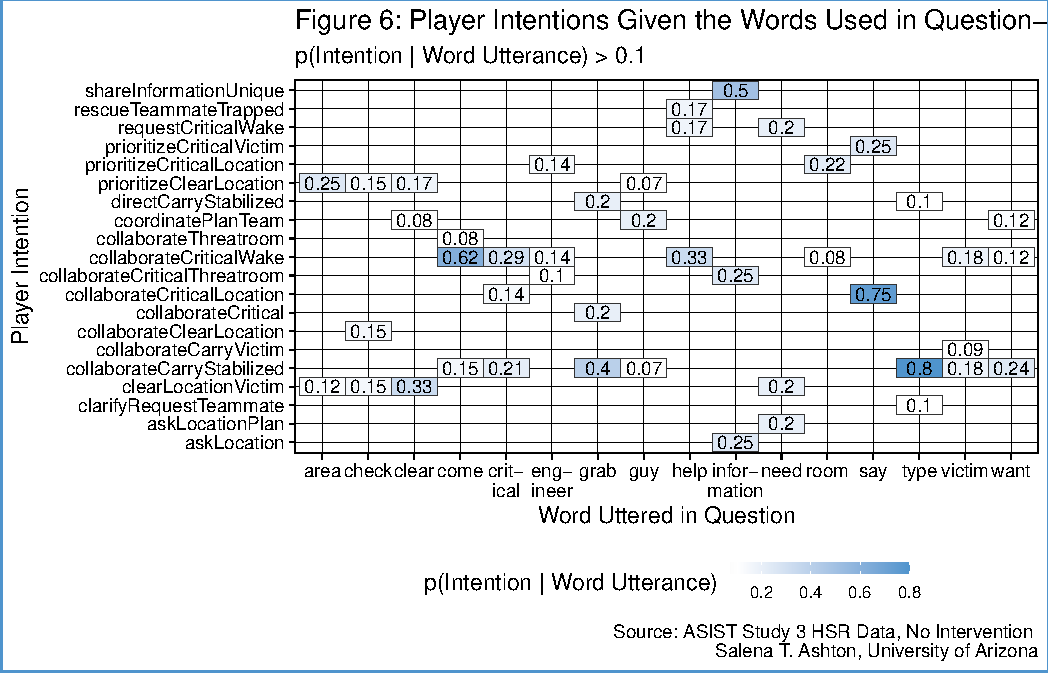
\includegraphics[width=0.9\textwidth]{../images/QuestionUtterances_Link_STA.pdf}}
    \caption{Players who work together tend to say  'come', 'say' (stemmed), 'type' or 'want.' When they work together to carry victims, they will most likely say 'type' (or mark) to identify the victim type.}
    \end{figure}

% p(Intent | Word Utterance)
\begin{figure}[h!]
    \centering
    \fbox{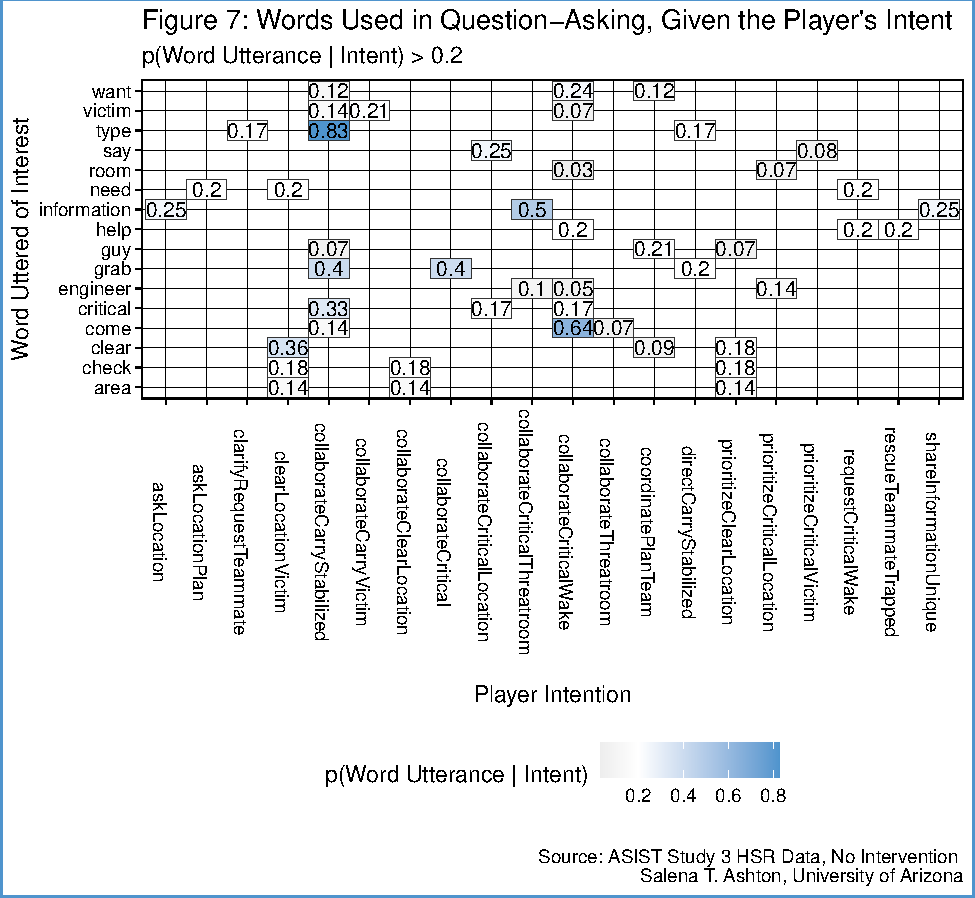
\includegraphics[width=0.9\textwidth]{"../images/Intent_to_Utterances_Link_STA.pdf"}}
    \caption{Non domain-specific words that show collaboration include 'say', 'type',
        or 'come'. }
\end{figure}
